\chapter{Arquitecturas de \textit{software}}

Según \cite{taylorSoftwareArchitectureFoundations2009}, la {\bf arquitectura de un sistema \textit{software}} es el conjunto de todas las decisiones de diseño principales que se toman durante la vida del sistema, aquellas que sientan las bases del desarrollo. \textcolor{red}{Se podría establecer un simil con los planos de construcción de un edificio.} Estas decisiones no solo se toman durante su concepción, si no también durante su desarrollo y posterior evolución.

La arquitectura afecta a todos los apartados del sistema: su estructura, funcionalidad, la implementación\dots Por ejemplo, una decisión de diseño principal que se suele tomar en las fases tempranas del desarrollo es la elección de la topología para la solución. Optar por desarrollar un servicio monolítico o una arquitectura basada en microservicios va a condicionar prácticamente todo el desarrollo. Desde el diseño, la implementación, el testeo, y sobre todo, el despliegue y operación. \textcolor{red}{Por tanto, es vital dedicar tiempo para definir la arquitectura en base a las necesidades de nuestro sistema.}

\section{Decisiones principales de diseño}

Las decisiones principales de diseño normalmente se resumen en comparativas entre distintas alternativas, cada una de ellas con sus ventajas e inconvenientes. Con el paso del tiempo, y con el avance del desarrollo, estas elecciones comienzan a asentarse, y se vuelven más dificiles de cambiar o rectificar.

Pueden tomarse en base a distintos criterios. Entre ellos podemos destacar: [Citation needed]

    \begin{itemize}
        \item \textbf{Requisitos del sistema:} a partir del dominio y las necesidades de nuestros usuarios, podemos deducir: la funcionalidad a implementar, las restricciones que debemos respetar y otras propiedades que debe poseer el sistema.

        \item \textbf{Arquitectura actual:} las decisiones tomadas previamente también condicionan las elecciones que se tomen más adelante. Cuanto más avanza el desarrollo, más se asientan las decisiones previas, y más dificil es rectificarlas.

        \item \textbf{Experiencia previa:} del desarrollo de este u otros sistemas. Podemos obtener métricas del funcionamiento y uso de nuestro sistema para informar decisiones futuras. \textcolor{red}{[Cita devops]}
    \end{itemize}

\section{Componentes de una arquitectura}

Según el estándar IEEE 42010-2011 \cite{ieeeStandard420102011Systems2011}, la arquitectura de un sistema es "\textit{un conjunto de conceptos o propiedades fundamentales, personificados por sus elementos, sus relaciones, y los principios que guían su diseño y evolución}". Nos provee de un marco de referencia común, de decisiones que nos nos provee con un vocabulario común, que nos permite describir sistemas

Por tanto, podemos describirla usando tres conceptos: \cite{perryFoundationsStudySoftware1992}

    \begin{itemize}
        \item \textbf{Componentes:} Son las piezas fundamentales que componen el sistema. Implementan la funcionalidad de la aplicación. Se utilizan para describir \textit{qué} partes conforman el sistema. Por ejemplo: un módulo, un servicio web...

        \item \textbf{Forma:} El conjunto de propiedades y relaciones entre los elementos o el entorno de operación. Describe \textit{cómo} está organizado el sistema. Por ejemplo: un servicio contacta con otro a través de una API.

        \item \textbf{Justificación:} Razonamiento o motivación de las decisiones que se han tomado. Responden al \textit{por qué} algo se hace de determinada forma. Normalmente no pueden deducirse a partir de los elementos y la forma, por lo que es necesario describirlos.

    \end{itemize}

\textcolor{red}{La arquitectura de un sistema puede contar con diferentes vistas, según aquel aspecto que deseemos resaltar. Por ejemplo, puede interesarnos más la interacción entre los componentes. O cosas por el estilo.}

Durante el diseño, para lidiar con la complejidad que pudiera alcanzar el sistema, solemos recurrir a descomponerlos usando diseños modulares: sistemas compuestos por unidades de funcionalidad que tienen una función específica. \cite{taylorSoftwareArchitectureFoundations2009} Estos elementos funcionales son los componentes. Dependiendo de las características de nuestro sistema, pueden tomar distintas formas: módulos dentro un mismo proceso, servicios distribuidos, etc.

Como hemos comentado antes, un sistema está conformado por \textbf{componentes} que implementan la funcionalidad de la aplicación. No suelen trabajar de forma aislada, si no que trabajan conjuntamente para realizar tareas más complejas. Por tanto, un aspecto clave es la integración y la interacción entre ellos. \cite{mehtaTaxonomySoftwareConnectors2000}

Para que dos o más componentes puedan interactuar, necesitamos definir un mecanismo de comunicación. Para ello, recurrimos a los \textbf{conectores}: se trata de elementos arquitectónicos que nos ayudan a diseñar y razonar sobre la comunicación entre componentes. Representan la transferencia de datos y de control entre componentes. En la figura \ref{fig:componentesEjemplo} mostramos una representación de la necesidad de comunicación entre dos componentes a través de un conector. No se ha especificado todavía ningún detalle sobre cómo se implementará. De esta forma, podemos estudiar la arquitectura y elegir los mecanismos adecuados para cada interacción del sistema. \cite{taylorSoftwareArchitectureFoundations2009}.

%% TODO: Los conectores son application-independent. No dependen de la funcionalidad de la aplicación.
%% TODO: Hablar de la cardinalidad de los conectores.

\begin{figure}[h!]
  \centering
  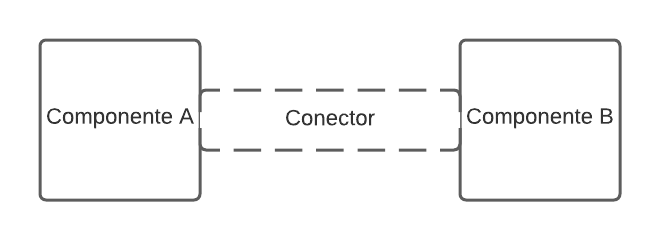
\includegraphics[scale=0.78]{02_arquitectura/images/conector}
  \caption{Ejemplo de comunicación de dos componentes a través de un conector.}
  \label{fig:componentesEjemplo}
\end{figure}

\textcolor{red}{A nivel de ¿diseño?}, los conectores están compuestos por uno o más \textbf{conductos} o canales de comunicación. A través de estos se lleva a cabo la comunicación entre los componentes. Hay una gran variedad de conductos posibles: comunicación interproceso, a través de la red, etc. Clasificamos los conectores según la complejidad de los canales que utilizan \cite{mehtaTaxonomySoftwareConnectors2000}:

\begin{itemize}
    \item \textbf{Conectores simples}: solo cuentan con un conducto, sin lógica asociada. Son conectores sencillos. Suelen estar ya implementados en los lenguajes de programación. Por ejemplo: una llamada a función en un programa o el sistema de entrada / salida de ficheros.

    \item \textbf{Conectores complejos}: cuentan con uno o más conductos. Se definen por composición a partir de múltiples conectores simples. Además, pueden contar con funcionalidad para manejar el flujo de datos y/o control. Suelen utilizarse importando \textit{frameworks} o librerias. Por ejemplo: un balanceador de carga que redirige peticiones a los nodos.
\end{itemize}

Por tanto, una vez hemos decidido que dos componentes deben comunicarse, es momento de evaluar cuál es el mecanismo de comunicación más adecuado. Para ello, podemos consultar la taxonomía de conectores de \cite{mehtaTaxonomySoftwareConnectors2000}. Basándonos en nuestros requisitos, la arquitectura ya definida, y los mecanismos de despliegue que queremos usar, elegimos el conector más adecuado.

\section{Arquitectura de la solución}

Como comentamos en el \autoref{chap:introduccion}: \nameref{chap:introduccion}, el objetivo del trabajo es adaptar un servicio monolítico para que funcione como un sistema distribuido basado en microservicios. Se trata de un cambio arquitectonico importante. Por ello, queremos diseñar una solución ingenieril teniendo en cuenta las particularidades del sistema.

Este servicio implementa un \textbf{bucle de control}, útil para dotar a un sistema con capacidades de computación autonoma. Especificamente, sigue la arquitectura del bucle MAPE-K\cite{ArchitecturalBlueprintAutonomic2006,fonsServiciosAdaptivereadyPara2021}, que mostramos en la figura \ref{fig:bucle-mapek2}. El objetivo de partida fue separar cada uno de los componentes del bucle en microservicios independientes.  \textcolor{red}{AÑADIR IMAGEN EJEMPLO DEL BUCLE DESCOMPUESTO EN MICROSERVICIOS. BUSCAR REFERENCIAS DE LIBROS SOBRE DIVIDIR MONOLITOS.}

\begin{figure}[h]
  \centering
  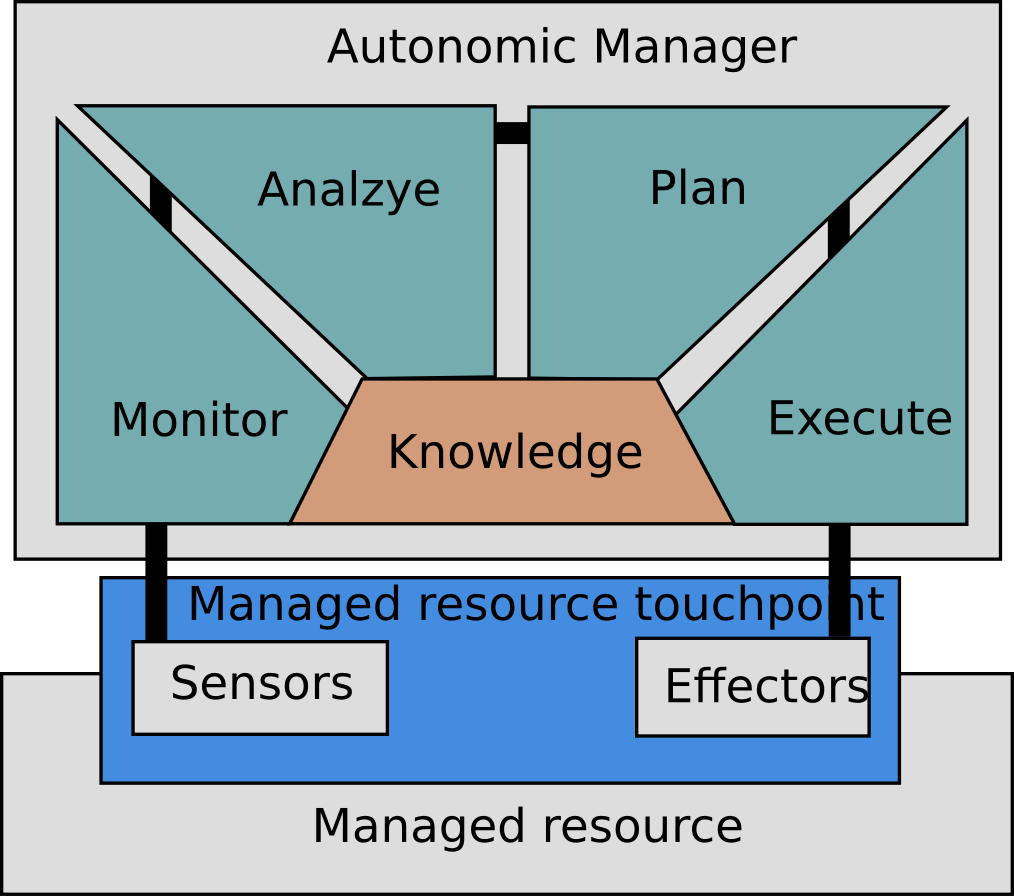
\includegraphics[scale=0.6]{01_introduccion/images/bucle-mape-k.png}
  \caption[Arquitectura de un Bucle MAPE-K.]{Arquitectura de un Bucle MAPE-K.\footnotemark}
  \label{fig:bucle-mapek2}
\end{figure}

% TODO: Cambiar por otra imagen sin typos.
\footnotetext{Obtenido de: \url{https://wwwvs.cs.hs-rm.de/vs-wiki/index.php/(WS12-01)_Cloud/Dokumentation}}

\textcolor{red}{Combinar con párrafo anterior: Actualmente, el sistema es un servicio monolitico que está muy acoplado a la solución. Queremos desacoplarlo para que pueda usarse la misma infraestructura para varios sistemas (\textit{multi-tennancy})}.

\subsection{Distribución de los componentes \textcolor{red}{TODO: MUY INCOMPLETO}}

Por suerte, partimos de un sistema existente, con una arquitectura bien definida y documentada. Conociamos el rol de los componentes del servicio y sus requisitos. Asi que, el primer problema al que nos enfrentamos estaba relacionado con la distribución de los servicios. ¿Cómo definimos las fronteras entre cada uno de ellos?

Una vez determinadas las "fronteras" entre los microservicios, hemos definido los componentes de nuestro sistema. Asi que, el primer problema al que nos enfrentamos estaba relacionado con la comunicación: si separamos las distintas etapas del bucle en microservicios, ¿cómo hacemos para que se comuniquen? Hay que tener en cuenta que estos pueden estar desplegados y replicados en distintas máquinas.

Por la descripción de ambos componentes, vemos que existe una clara división de dominios y responsabilidades. Esto nos ayuda a determinar que ambos componentes pueden desplegarse por separado. \textcolor{red}{REFERENCIA 'Building Microservices' Sam Newman}

\begin{figure}[h]
  \centering
  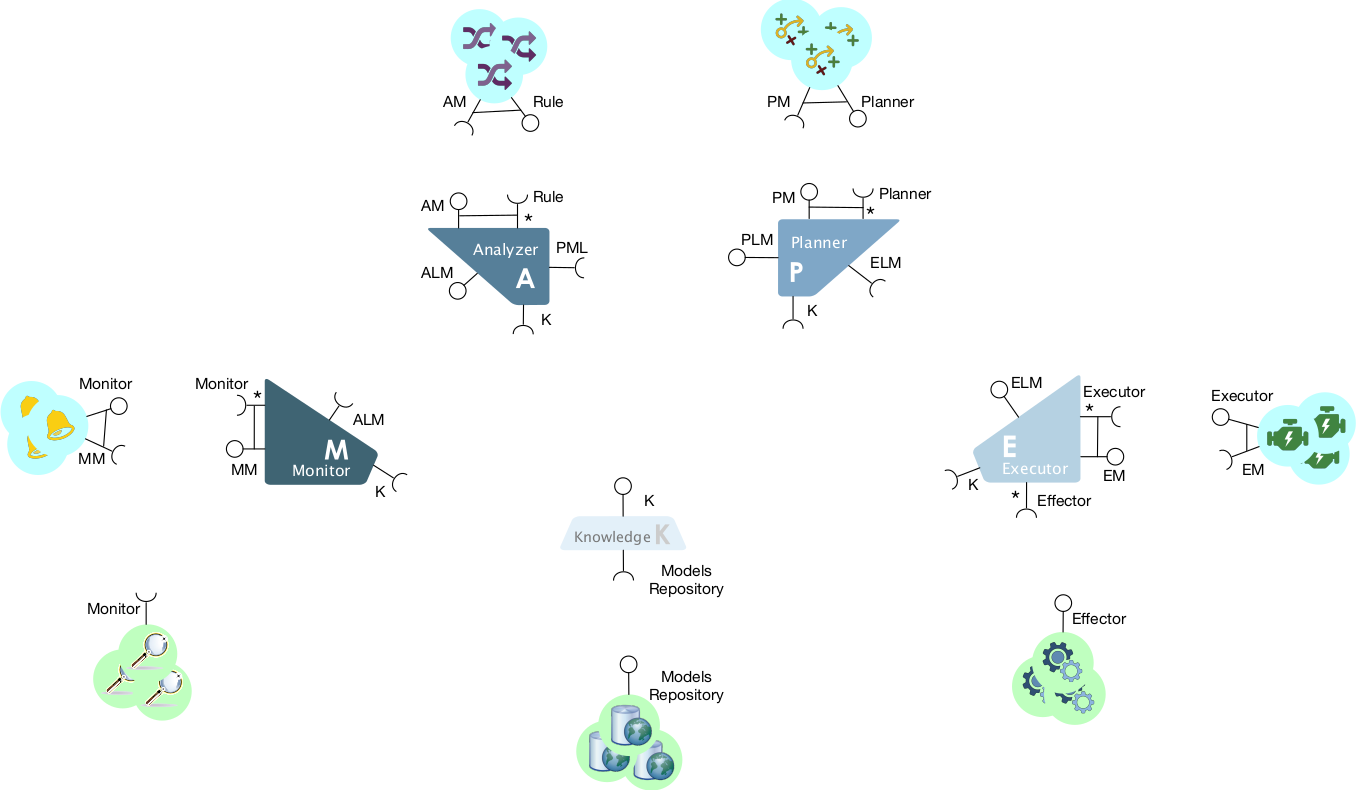
\includegraphics[scale=0.3]{02_arquitectura/images/mape-k-microservices}
  \caption{Diagrama con los componentes que forman nuestra arquitectura distribuida}
  \label{fig:mape-k-microservices}
\end{figure}

\textcolor{red}{En este caso, ponian como ejemplo un estilo arquitectónico que se llama C2 (components and connectors, creo) . La idea era tener capas o niveles de microservicios. Un microservicio en una capa concreta solo pueden contactar con sus vecinos (inmediatamente superior e inmediatamente inferior). Dentro del mismo nivel no pueden contactar entre ellos. Según la dirección de la comunicación, se utilizan mecanismos distintos:}

\begin{itemize}
  \item \textbf{Peticiones}: Un microservicio de más abajo en la jerarquía (o más externo), se comunica con un vecino que está más arriba. Por ejemplo, sería el caso de cuando el servicio de monitorización escribe una propiedad en el servicio de conocimiento.

  \item \textbf{Notificaciones}: Un microservicio de más arriba en la jerarquía (o mas interno), se comunica con un vecino que está por debajo de él. Por ejemplo, cuando el servicio de conocimiento notifica al servicio de análisis que ha cambiado una propiedad.
\end{itemize}

He encontrado una imagen que lo describe más o menos:

\begin{figure}[h]
  \centering
  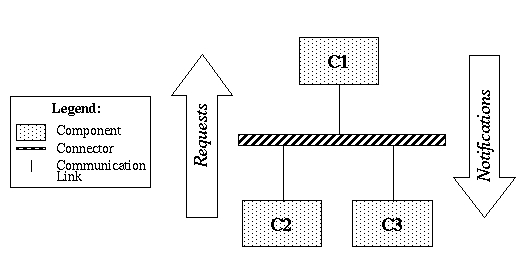
\includegraphics[scale=0.45]{02_arquitectura/images/c2SampleArch}
  \caption{Ejemplo del estilo arquitectónico C2 (\textit{Components and Connectors}). \cite{UCISoftwareArchitecture}}
  \label{fig:C2-arch-example}
\end{figure}

Mi propuesta entonces sería inspirarnos un poco en esta aproximación. Asi aprovechamos para dividir los microservicios en niveles y elegir los mecanismos para cada tipo de comunicación.

Yo distinguiría entre 4 niveles, desde más externo a más interno:

\begin{itemize}
  \item \textbf{Más externo}: Sondas y Efectores. Son los elementos que ya tienen más contacto con el sistema gestionado por el bucle. Cuanto menos esté acoplado el bucle a ellos mejor.

  \item \textbf{Nivel de solución}: En esta capa se encuentran los microservicios específicos a una solución concreta. En el ejemplo que te mostré el otro día, sería el servicio de Room Monitor, que monitoriza la temperatura de una habitación

  \item \textbf{Nivel del bucle}: Aquí se encuentran los servicios del propio bucle: servicio de monitorización, análisis, planificación y ejecución. Esta capa no debería tener dependencias con los microservicios de la solución. Es justo lo queríamos abordar en este trabajo.

  \begin{itemize}
    \item También se aprecia algo que implementé en mi solución: el servicio de monitorizacion hace de intermediario entre los monitores de la solución y el conocimiento. No se accede directamente a estas propiedades.
  \end{itemize}

  \item \textbf{Conocimiento}: Es la capa más interna y la base de la arquitectura. Todos los microservicios de la capa del bucle dependen de ella para funcionar.

\end{itemize}

Me he basado en el diagrama típico de Clean Architecture para representar un poco la idea:

\begin{figure}[h]
  \centering
  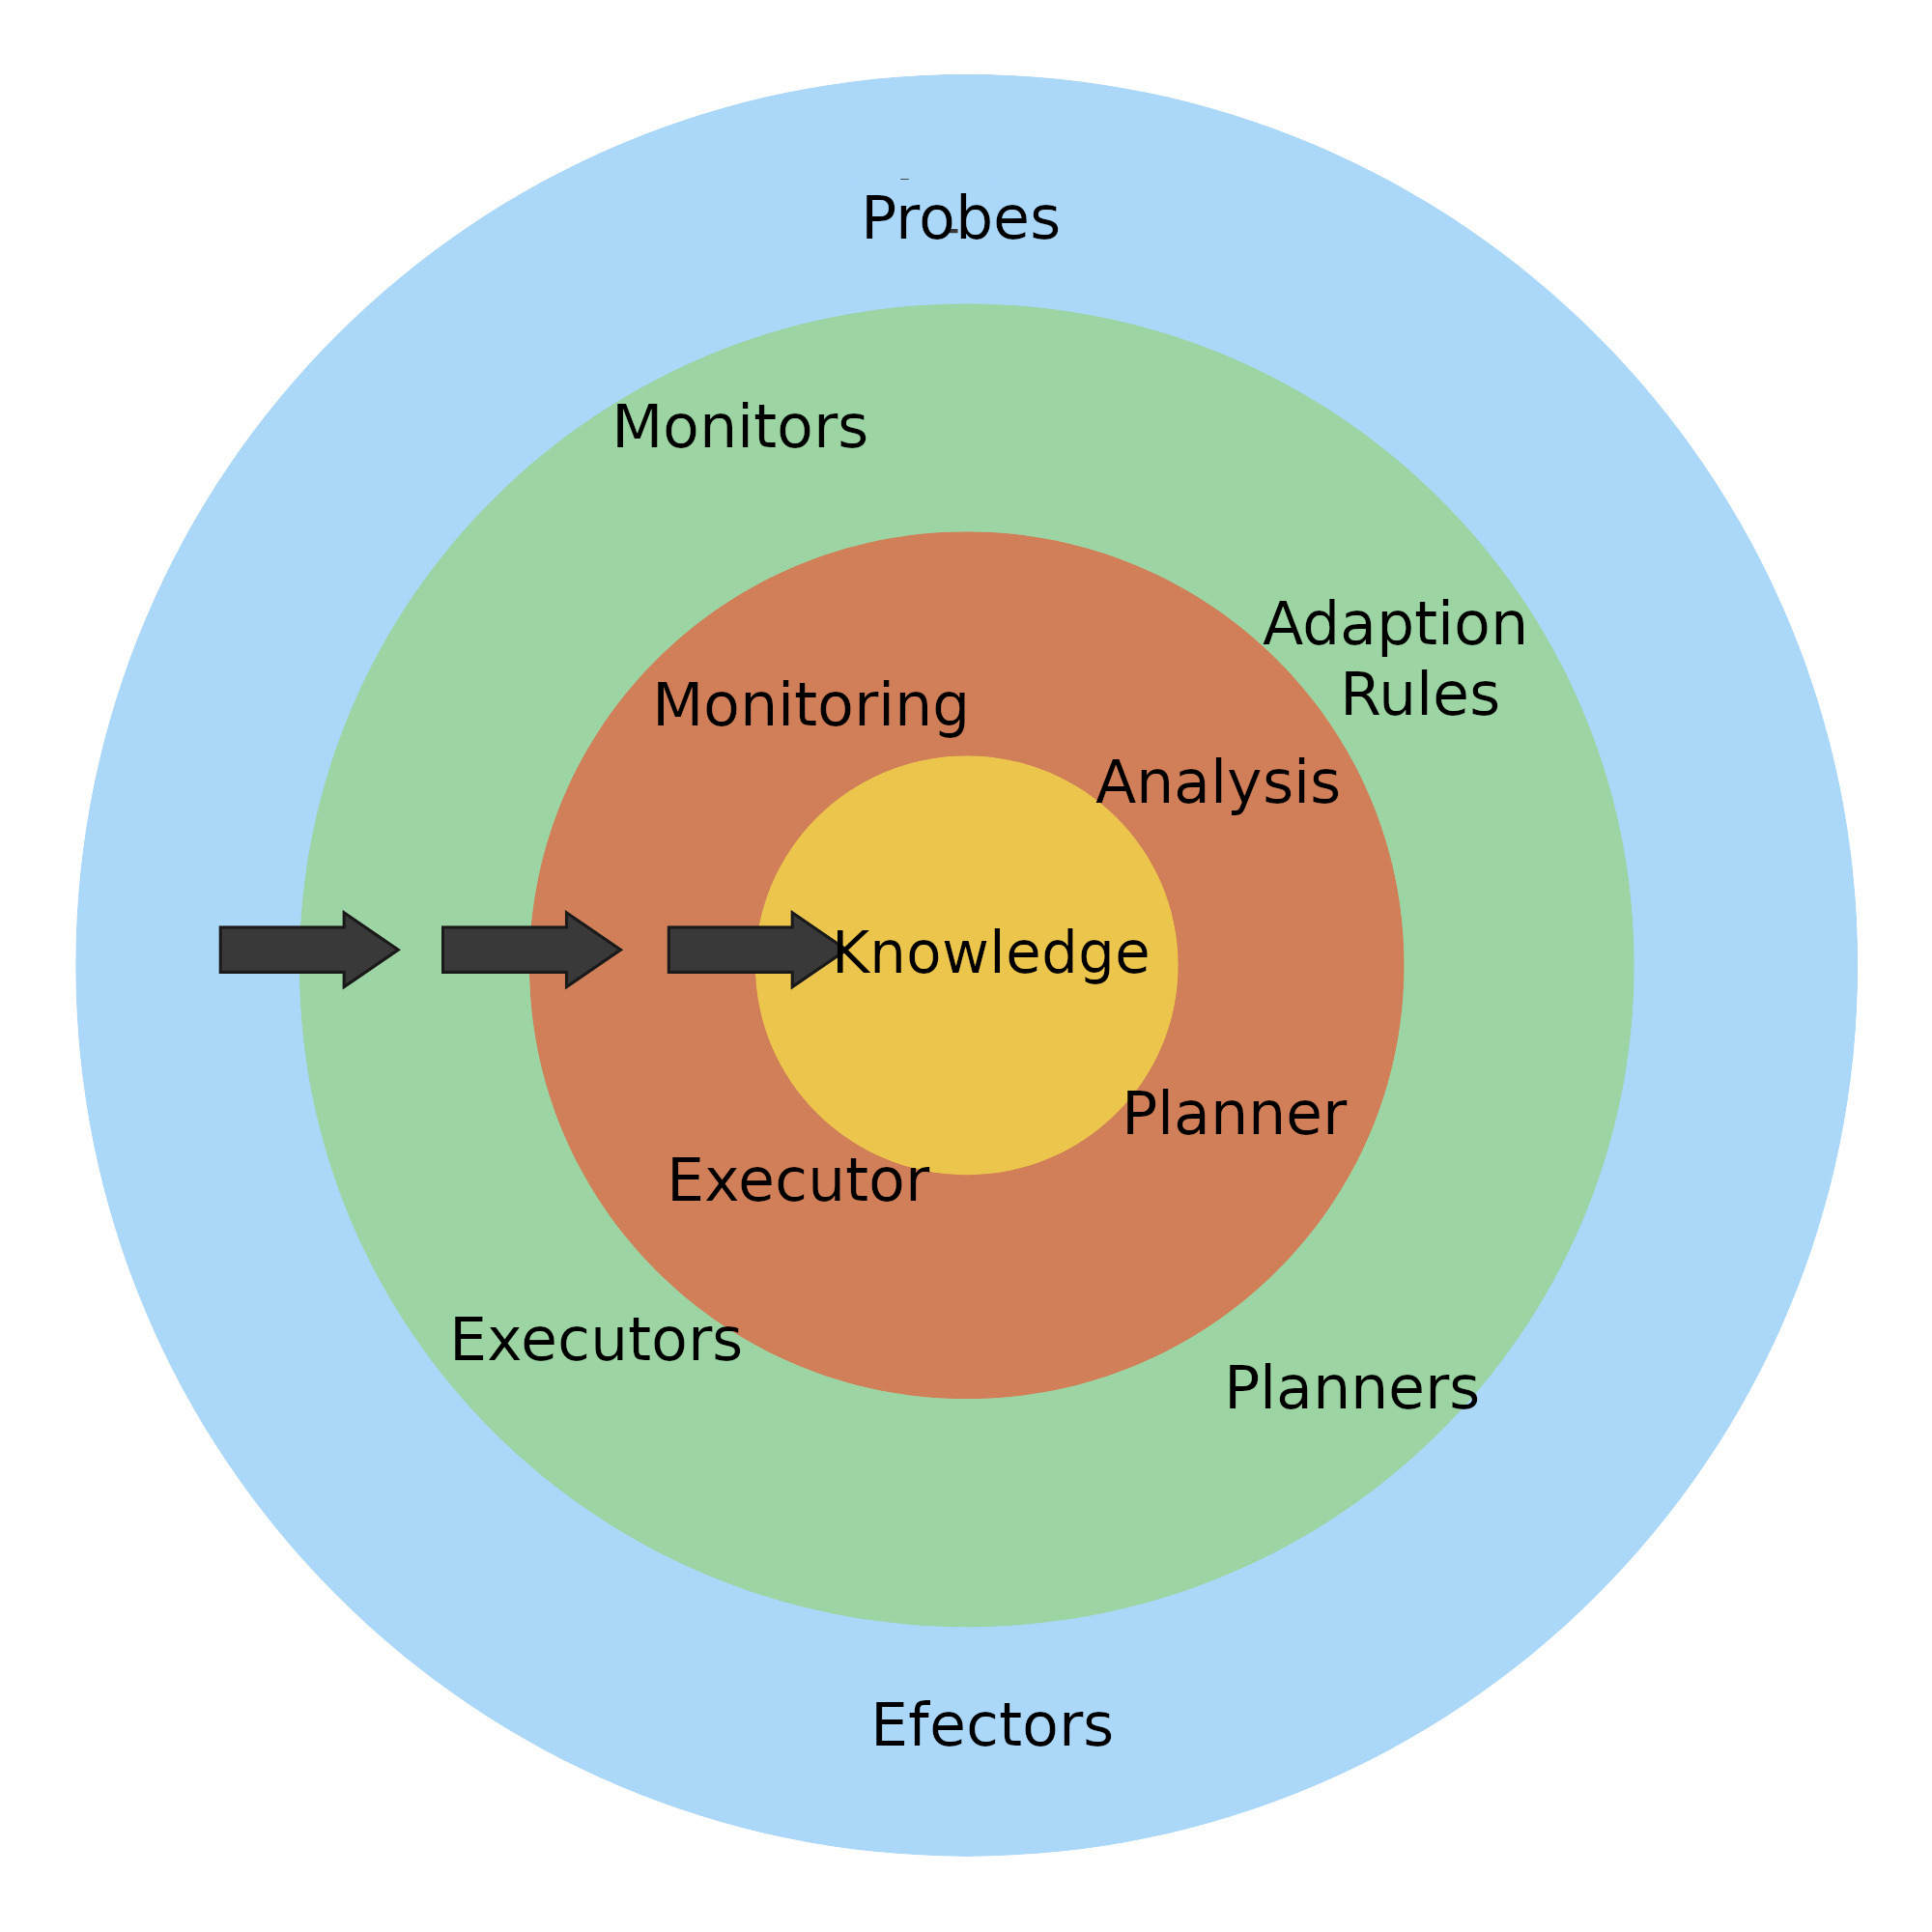
\includegraphics[scale=0.45]{02_arquitectura/images/clean-arch-2-MAPEK-style}
  \caption[Representación de nuestra propuesta arquitectónica. Inspirado en Arquitectura Limpia (\textit{Clean Architecture}).]{Representación de nuestra propuesta arquitectónica. Inspirado en Arquitectura Limpia (\textit{Clean Architecture}). \footnotemark }
  \label{fig:clean-mapek-architecture}
\end{figure}

\footnotetext{Imagen original de arquitectura limpia obtenida de: \url{https://threedots.tech/post/ddd-cqrs-clean-architecture-combined/}}


En el dibujo, las flechas de "fuera hacia adentro" representarían las Peticiones (o requests). Las notificaciones irían en sentido contrario.

Mi idea entonces es definir dos tipos de conectores:

\begin{itemize}
  \item \textbf{Peticiones}: Utilizamos la estrategia que ya definimos en el hito anterior. Los servicios ofrecen APIs REST con una serie de operaciones. Las peticiones fluyen de microservicios más externos a los más internos, mediante llamadas HTTP.

  \begin{itemize}
    \item Por ejemplo, en el hito anterior: Probe -> Monitor -> Monitoring Service -> Knowledge

    \item Utilizamos OpenAPI para autogenerar clientes, así facilitamos la implementación de los clientes en cualquier lenguaje
  \end{itemize}

  \item \textbf{Notificaciones}: En este caso optaría por usar brokers de mensajería (o algo parecido), de forma que los microservicios de capas más internos notifican a las más externas, sin necesidad de acoplarse directamente. Cada capa estaría suscrita a los eventos de la que esté por debajo de ella. Por ejemplo: Analysis Service se suscribe a Knowledge, las Reglas de Adaptación se suscriben al Analysis Service, etc.

  \begin{itemize}
    \item Seguiría un poco la filosofía que comentamos hace un tiempo para independizar el módulo de análisis del de monitorización.

    \item Podríamos investigar la idea que has comentado, de un conector que abstraiga al cliente de esta suscripción a una cola de mensajería. A esto no le he dado muchas vueltas aun.
  \end{itemize}

\end{itemize}

\subsection{Comunicación entre componentes}

Una vez determinadas las ''fronteras'' entre los microservicios, hemos definido los componentes de nuestro sistema. El siguiente problema al que nos enfrentamos fue la comunicación: si separamos las distintas etapas del bucle en microservicios, ¿cómo hacemos para que se comuniquen? Debemos tener en cuenta que estos pueden estar desplegados en máquinas distintas.

Comenzamos entonces la búsqueda de los conectores más apropiados para cada par de componentes. Seguimos la estrategia descrita en \cite{taylorSoftwareArchitectureFoundations2009} y consultando patrones de comunicación en sistemas distribuidos descritos en \cite{newmanBuildingMicroservicesDesigning2021}. \textcolor{red}{AMPLIAR} Comenzamos eligiendo qué dos componentes queremos conectar.

Tomemos por ejemplo la comunicación entre el servicio de monitorización (\textit{monitoring service}) y el servicio de conocimiento (\textit{knowledge service}). Recordemos que el servicio de conocimiento almacena todas las propiedades de adaptación. El resto de servicios necesitan consultar y actualizarlas durante su funcionamiento. En la figura \ref{fig:monitor-knowledge-initial} representamos inicialmente ambos componentes y un conector, sin especificar de qué tipo será.

\begin{figure}[h]
  \centering
  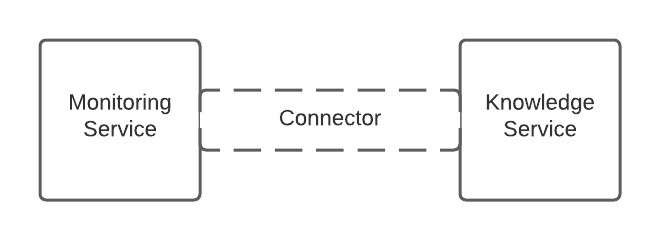
\includegraphics{02_arquitectura/images/Monitor-Knowledge-Initial-Connector}
  \caption{Boceto inicial: queremos conectar el servicio de monitorización con la base de conocimiento para poder leer propiedades de adaptación.}
  \label{fig:monitor-knowledge-initial}
\end{figure}

El siguiente paso es identificar qué interacciones debe existir entre ambos componentes. En este caso, el servicio de monitorización debe contactar con el servicio de conocimiento para leer y actualizar el valor de las propiedades. Por tanto, existen operaciones de lectura y escritura de los datos.

Ahora, debemos identificar qué \textbf{tipos de conector} serían adecuados para nuestros componentes. Sabiendo que hemos optado por una arquitectura distribuida, la elección se simplifica: los servicios pueden estar desplegados en máquinas distintas, por tanto el paso de mensajes será a través de la red.

Sabiendo esto, en lugar de recurrir a la taxonomía que lista \cite{mehtaTaxonomySoftwareConnectors2000}, optamos por consultar las estrategias de comunicación habituales para sistemas distribuidos descritas en \cite{newmanBuildingMicroservicesDesigning2021}. Se trata de cuatro mecanismos distintos: Invocación a métodos remotos (\textit{Remote Procedure Call}), APIs REST, consultas con GraphQL o \textit{brokers} de mensajería. Tuvimos que evaluarlos mediante un análisis de \textit{trade-offs} para determinar las ventajas y desventajas de cada uno.

\begin{itemize}
  \item \textbf{Invocación de métodos remotos} o (\textit{\textbf{Remote Procedure Call}}): Se trata de un paradigma de objetos distribuidos. \cite{taylorSoftwareArchitectureFoundations2009} Nuestro programa interactúa con objetos que se encuentran en servidores remotos. \textcolor{red}{Suele implementarse con objetos que actúan como un \textit{proxy}: ofrecen una interfaz para que el cliente invoque sus funciones localmente. Estas funciones internamente realizan una llamada al servicio remoto, donde se encuentre este objeto.} El servidor remoto procesa la petición y nos devolverá un resultado. Así, abstraen al cliente de todo este proceso de comunicación.

  Estos \textit{proxies} suelen generarse a partir de un contrato, que define que operaciones ofrecen estos objetos.
  Existen varios protocolos que implementan este mecanismo, como Java RMI, gRPC o SOAP.

  \begin{itemize}
    \item \textbf{Ventajas}:
    \begin{itemize}
      \item Permite la distribución del procesamiento del sistema.

      \item Abstrae al cliente de esta interacción a un servidor remoto. No tenemos que implementar la interacción con el servidor.

      \item Al haber un contrato definido, podemos generar los \textit{proxies} o clientes basados en este contrato. Por ejemplo: SOAP con WDSL o gRPC.
    \end{itemize}

    \item \textbf{Desventajas}:
    \begin{itemize}
      \item No se puede abstraer completamente al cliente de las llamadas a través de la red. Pueden darse errores que no ocurrirían durante una invocación de un método sobre un objeto local. Por ejemplo, que el servidor no esté disponible. \cite{jausovecFallaciesDistributedSystems2020}

      \item Si adoptamos sistemas como Java RMI, nuestro sistema se acopla a esa tecnología concreta. \cite{newmanBuildingMicroservicesDesigning2021}. Nos resta flexibilidad en cuanto a qué otras tecnologías podemos utilizar en nuestra arquitectura.

      \item El cliente debe actualizarse y recompilarse con cada cambio en el esquema del servidor. Esto puede ser problemático para casos donde tenemos que desplegar una actualización para que nuestros clientes puedan continuar utilizando la aplicación.
    \end{itemize}
  \end{itemize}

  \item \textbf{\textit{Representational State Transfer} (REST)}: Se trata de un estilo arquitectónico basado en el estilo cliente - servidor, pero con ciertas restricciones adicionales. \cite{taylorSoftwareArchitectureFoundations2009} Su concepto principal son los \textbf{recursos}: cualquier elemento que pueda tener asociado un identificador (una URI). \cite{richardsonRESTfulWebServices2007} Sobre los recursos podemos ejecutar una serie de acciones definidas por el protocolo de comunicación. Normalmente, el protocolo es HTTP.

  \begin{itemize}
    \item \textbf{Ventajas}:

    \begin{itemize}
      \item \textbf{Escalable}:

      \item \textbf{\textit{Stateless}}: El servidor no mantiene el estado de la operación.

      \item \textbf{Interoperabilidad}: Ampliamente utilizado en servicios de Internet. Es ideal para que clientes externos contacten con nuestro sistema mediante peticiones síncronas. \cite{newmanBuildingMicroservicesDesigning2021}
    \end{itemize}
  \end{itemize}

  \begin{itemize}
    \item \textbf{Desventajas}:

    \begin{itemize}
      \item \textbf{Rendimiento}: El rendimiento es peor comparado con cualquier mecanismo RPC binario. La información serializada en XML o JSON es mayor que si estuviera en un formato binario.

      \item \textbf{Rendimiento}: El rendimiento es peor comparado con cualquier mecanismo RPC binario. La información serializada en XML o JSON es mayor que si estuviera en un formato binario.
    \end{itemize}
  \end{itemize}

  \item \textbf{GraphQL}\footnote{Página oficial: \url{https://graphql.org/}}: Se trata de un protocolo para que un cliente pueda hacer consultas personalizadas sobre los datos de un servidor. No necesitan que haya sido implementado con lógica asociada. De esta forma, se puede reducir la cantidad de peticiones a través de la red que se necesita ejecutar para obtener la misma información.

  \begin{itemize}
    \item \textbf{Ventajas}:

    \begin{itemize}
      \item \textbf{Ideal para móviles}: Gracias a que reduce la cantidad de llamadas, es ideal para entornos donde queremos optimizar el uso de datos.

      \item \textbf{Rendimiento}: Ofrece un mayor rendimiento comparado con otras alternativas que no ofrezcan un endpoint ya implementado. Y debamos obtener la misma información por composición, haciendo varias llamadas.
    \end{itemize}
  \end{itemize}

  \begin{itemize}
    \item \textbf{Desventajas}:

    \begin{itemize}
      \item \textbf{Exponemos datos a la red}:

      \item \textbf{Problemas de rendimiento}: El cliente puede hacer consultas muy pesadas que penalicen el rendimiento de la base de datos sobre la que opera nuestro servicio.
    \end{itemize}
  \end{itemize}

  \item \textbf{\textit{Brokers} de mensajería}:
\end{itemize}

\textcolor{red}{De estas cuatro opciones, podemos descartar inmediatamente la opción de GraphQL. Se trata de un conector más orientado a las consultas de datos. Nosotros necesitamos ejecutar escrituras de los valores de las propiedades. Aunque podría implementarse para el servicio de las lecturas, no preveemos que las consultas de las propiedades requieran de agregación de datos. Simplemente se obtiene el valor de una propiedad.}

\textcolor{red}{Por otro lado, una de nuestras prioridades es la interoperabilidad, para que cualquier microservicio que implemente esta API peuda comunicarse con nuestro servicio. Finalmente, queríamos que la comunicación fuese síncrona a la hora de solicitar propiedades, por lo que nos terminamos decantando por REST sobre HTTP.}

Aun así, queríamos aprovechar algunas de las ventajas que ofrece RPC para simplificar la integración de nuestra API con las librerias clientes.

\textdagger{\textcolor{red}{A continuación, debemos identificar qué \textbf{rol} debe jugar este conector. Se trata de cubrir la \textbf{comunicación} entre dos componentes: necesitamos enviar y recibir datos del servicio de persistencia. También detectamos que es necesaria la \textbf{coordinación} entre los componentes. Por ejemplo, para la lectura de propiedades debemos contactar con otro servicio, y esperar su respuesta. Hay por tanto una transferencia de control entre ellos. Respecto al resto de roles, de momento no hemos detectado necesidad de conversión o facilitación.}}

En este caso, hemos optado por una mezcla de RPC implementado sobre HTTP. No se trata de una implementación del todo rest. Pero de esta forma, podíamos evitar acoplarnos a una tecnología concreta, como describe el libro. Nos parecía más razonable que el monitor exponga directamente una API HTTP pública. De esta forma, podríamos explotar el uso de OpenAPI, un DSL para describir APIs que explicaremos a continuación.

Así, mejoramos la compatibilidad con cualquier cliente, y nos daba más flexibilidad.

Ya tenemos la parte de la API, expuesta por el servidor. Ahora nos queda la parte del cliente. ¿Cómo contactamos desde el monitor con la API? Implementamos las llamadas directamente con un cliente HTTP? Esto será muy costoso de mantener, y no será resiliente a los cambios. Será muy complicado.

Por suerte, a partir de la especificación OpenAPI, podemos generar un componente que haga de cliente de la solución. Este cliente hace de Proxy y nos abstraen de la lógica para establecer la conexión, el protocolo de comunicación, formato de los mensajes, etc.

%% TODO: Justificar división del dominio del bucle de control. Hay que hacer un diagrama que explique cómo queremos separar el dominio (probe y monitor) del propio bucle de control.

\begin{figure}[h]
  \centering
  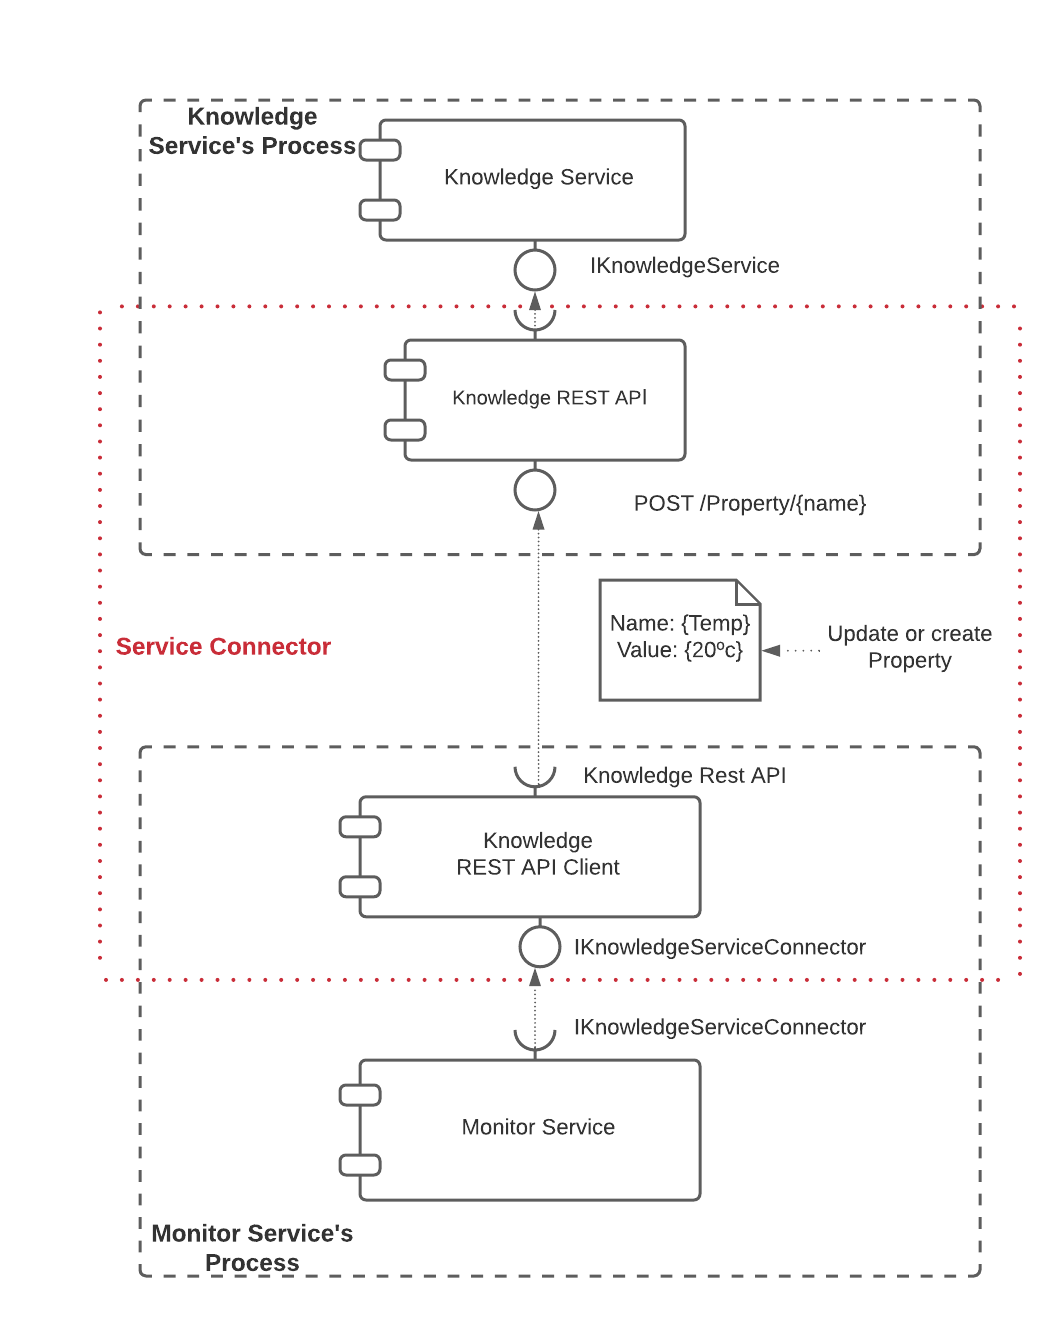
\includegraphics[scale=0.75]{02_arquitectura/images/Monitor-Knowledge-Connector}
  \caption{Diseño del conector usando implementación Cliente - Servidor}
  \label{fig:monitor-knowledge-connector}
\end{figure}

\pagebreak

\subsection{Open API}

\begin{wrapfigure}{r}{0.35\linewidth}
  % \vspace{15pt}
  
\includegraphics[scale=0.34]{02_arquitectura/images/openapi-logo}
  \centering
  % \vspace{15pt}
\end{wrapfigure}

OpenAPI\footnote{Open API specification: \url{https://spec.openapis.org/oas/latest.html}} es un lenguaje estándar para describir APIs implementadas sobre el protocolo HTTP. Es un \textit{domain specific language} que podemos utilizar para describir APIs de nuestras aplicaciones

Para el desarrollo de este trabajo, hemos optado por utilizar conectores basados en APIs REST. Nos permitía utilizar mecanismos ya presentes en los microservicios que queríamos desarrollar, y que fueran más homogéneos.
Para facilitar la compatibilidad de los microservicios, y facilitar el desarrollo de nuevos microservicios, hemos decidido usar la especificación OpenAPI.

La principal ventaja que nos ofrecía OpenAPI era la posibilidad de generar código a partir de la especificación. Permite generar código tanto del cliente como del servidor. De esta forma, podíamos implementar nuestra API genérica en un lenguaje . En este caso, se decidió utilizar conjuntamente el lenguaje C\# junto con el framework ASP.NET Core, para implementar los microservicios iniciales.

A partir de estos microservicios, podemos exportar la especificación de OpenAPI, haciendo uso de los endpoints, atributos y comentarios. Por ejemplo, en este endpoint del servicio de monitorización, vemos cómo obtiene una propiedad del servicio de conocimiento.

Podemos observar cómo el método está decorado con atributos que describen el tipo de respuesta que produce, según el código de respuesta HTTP. Estos comentarios se utilizan en la generación de la especificación para obtener mejor implementación

Después, haciendo uso de las librerías de generación de código de OpenAPI.
